
\chapter{Introduction}
\label{cha:1_Introduction}

% the code below specifies where the figures are stored
\ifpdf
    \graphicspath{{1_introduction/figures/PNG/}{1_introduction/figures/PDF/}{1_introduction/figures/}}
\else
    \graphicspath{{1_introduction/figures/EPS/}{1_introduction/figures/}}
\fi


%-------------------------------------------------------------------------
%Chapter 1 contents:
%- Motivation of the research field: Context-aware systems -> LBS -> GNSS limitation -> Positioning techniques -> DR -> inertial PDR -> inertial PDR + wearables
%- Problem identification: smartphone not a wearable -> potentiality of wrist-worn wearables -> Problem: no wrist-worn PDRS
%- Goal of the thesis: tackle the problem -> how? Splitting it into sub-problems
%- Structure of the thesis
%-------------------------------------------------------------------------

Governments and companies are producing vast streams of data and require effective data analytics and machine learning methods to assist in making predictions and decisions promptly. One crucial aspect is the machine learning pipeline, which involves training a prepared dataset to construct a model and subsequently utilizing this model to predict new instance outputs. Figure \ref{fig:machine-old-senario} shows that the process entails fetching historical data from the database during the training phase to construct the machine learning model. Then, the system can input new instances from the database to predict the output.

\begin{figure}[!ht]
    \centering
    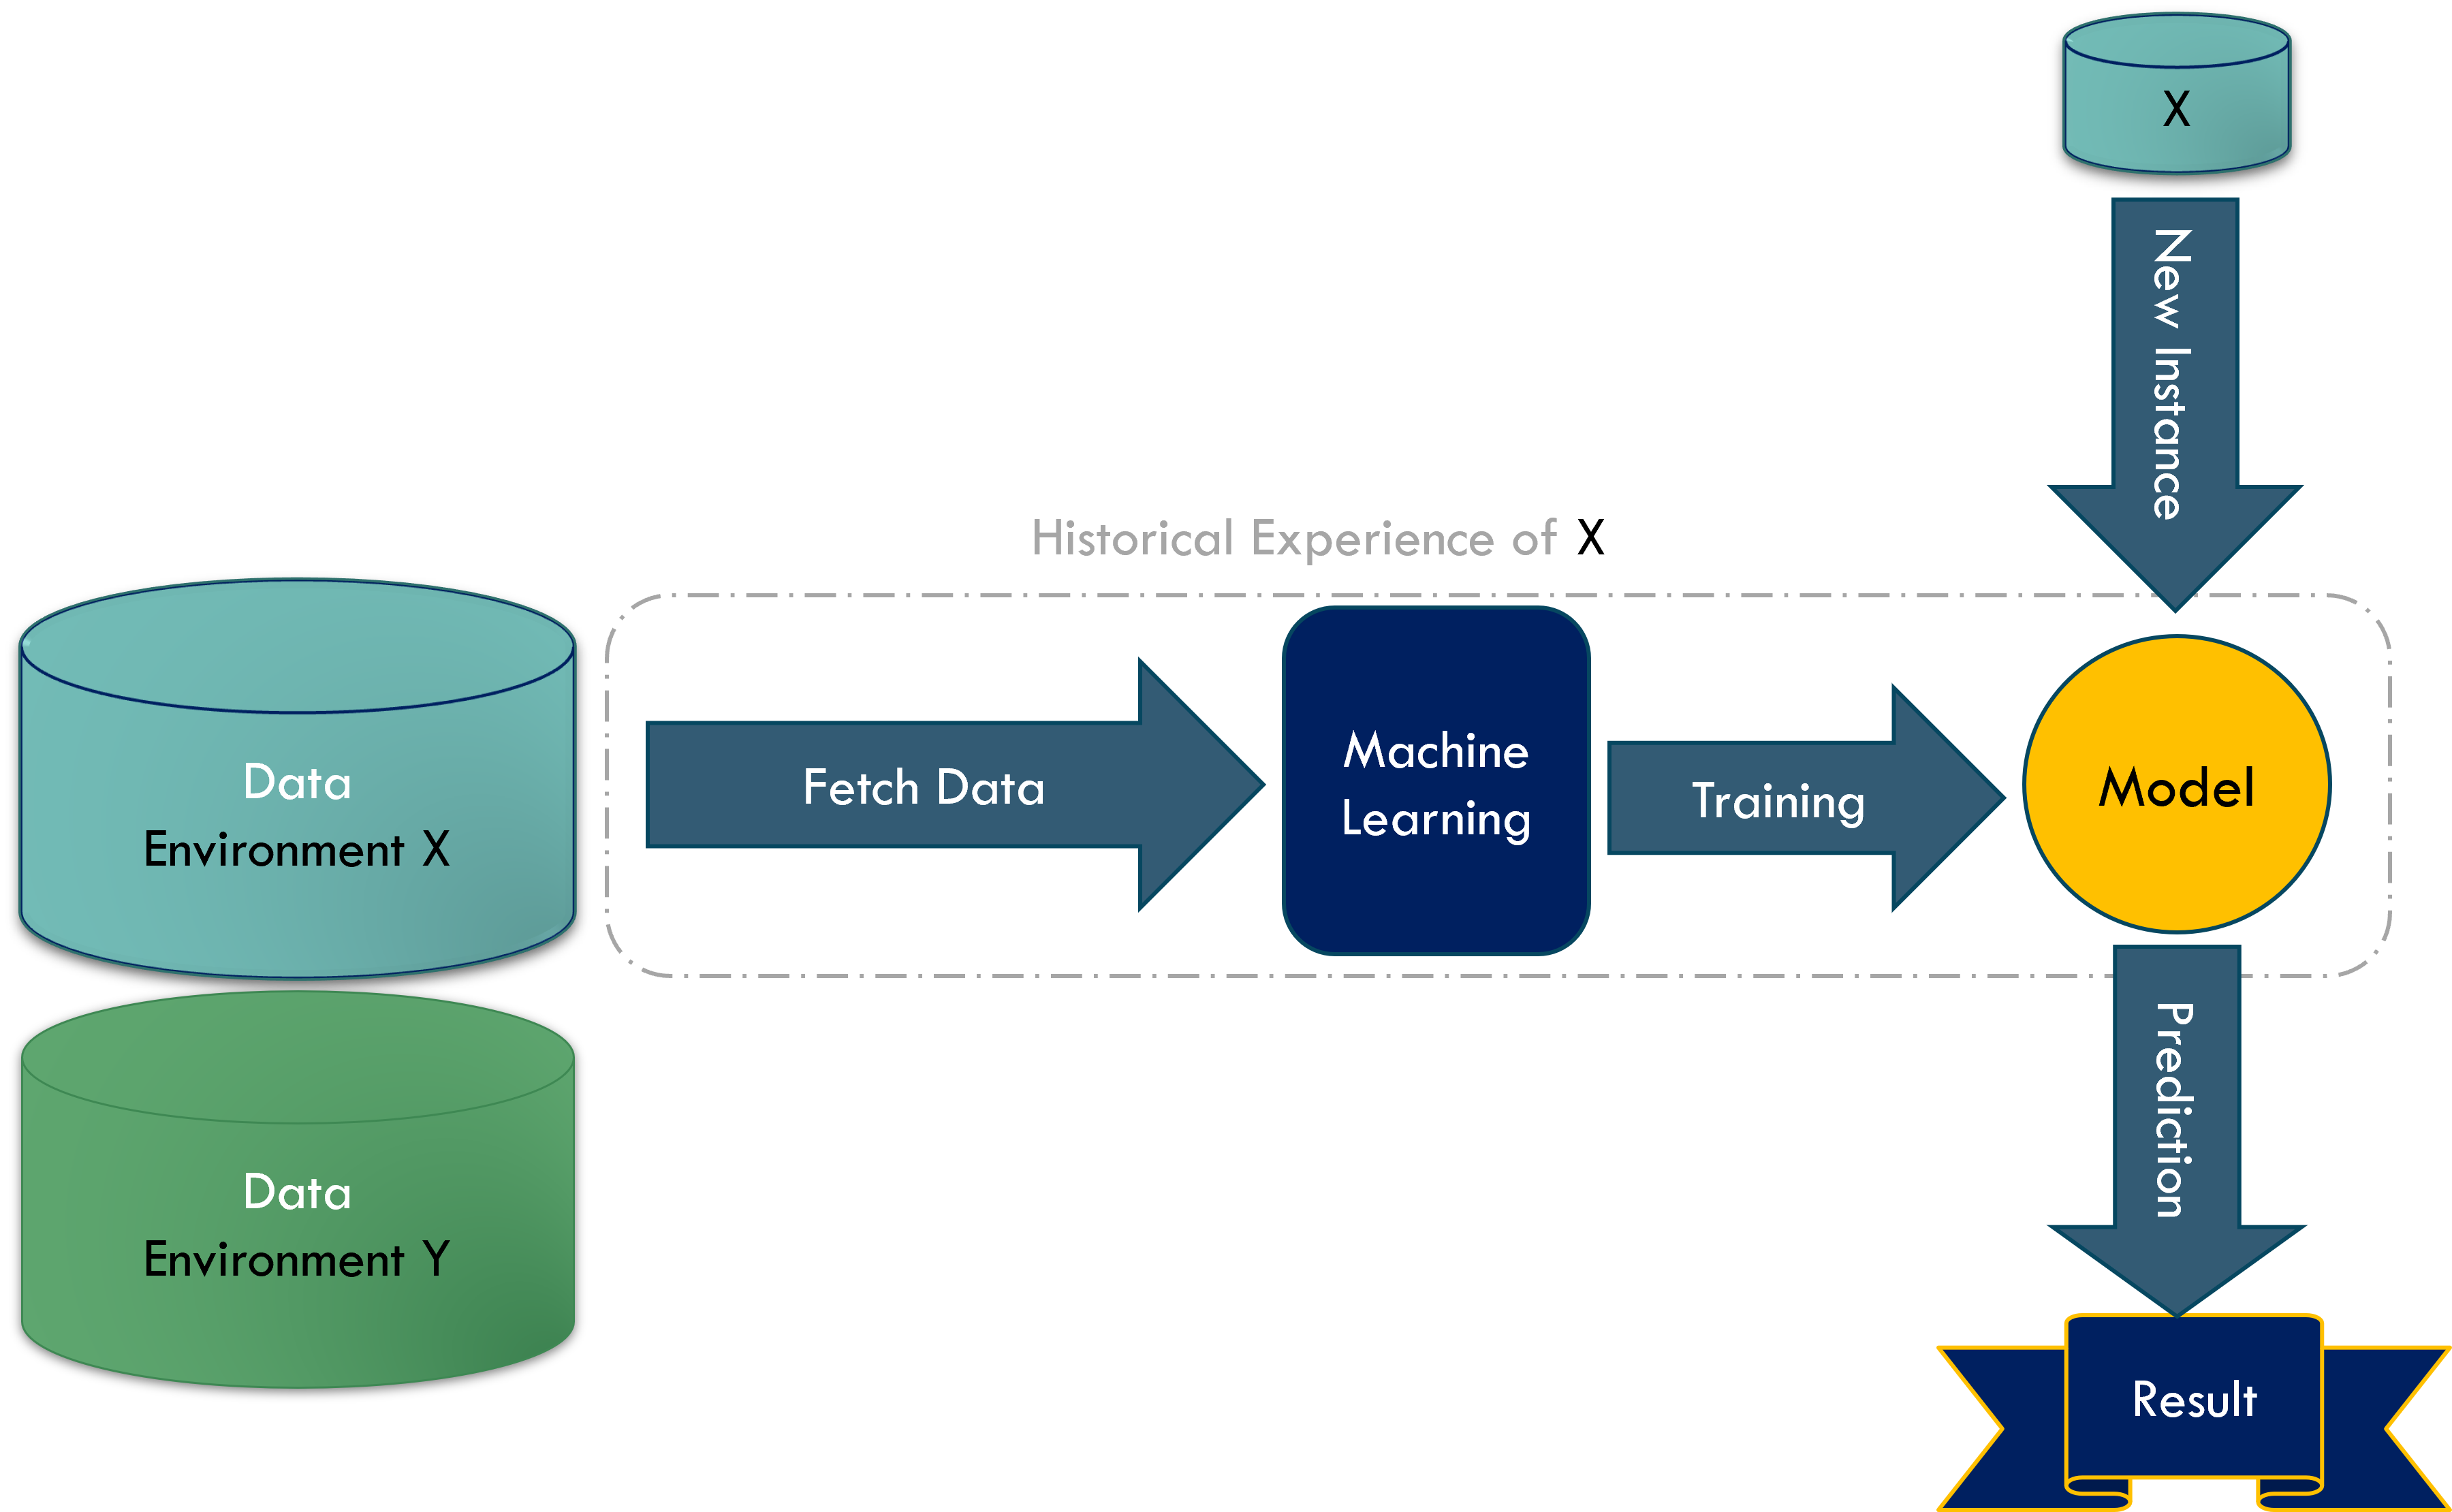
\includegraphics[width=.9\textwidth]{1_introduction/figures/PNG/machine_flow.png}
    \caption{Machine Learning Workflow for Environment X.}
    \label{fig:machine-old-senario}
\end{figure}

Nevertheless, when endeavoring to forecast outcomes for fresh instances sourced from an alternative database, as illustrated in Fig. \ref{fig:machine-new-senario}
, there frequently emerges a conspicuous decline in accuracy. This disparity accentuates the imperative for model developers to intervene and rectify the issue. Addressing this, developers must adjust and retrain the model utilizing datasets from the new environment to ameliorate performance. This iterative process aims to refine the model's precision and ensure its efficacy across diverse contexts, thereby bolstering the reliability of decision-making and predictive capabilities. To confront this challenge, the field of auto machine learning endeavors to facilitate online updates to the model without necessitating direct intervention from developers for modification.

\begin{figure}[!ht]
    \centering
    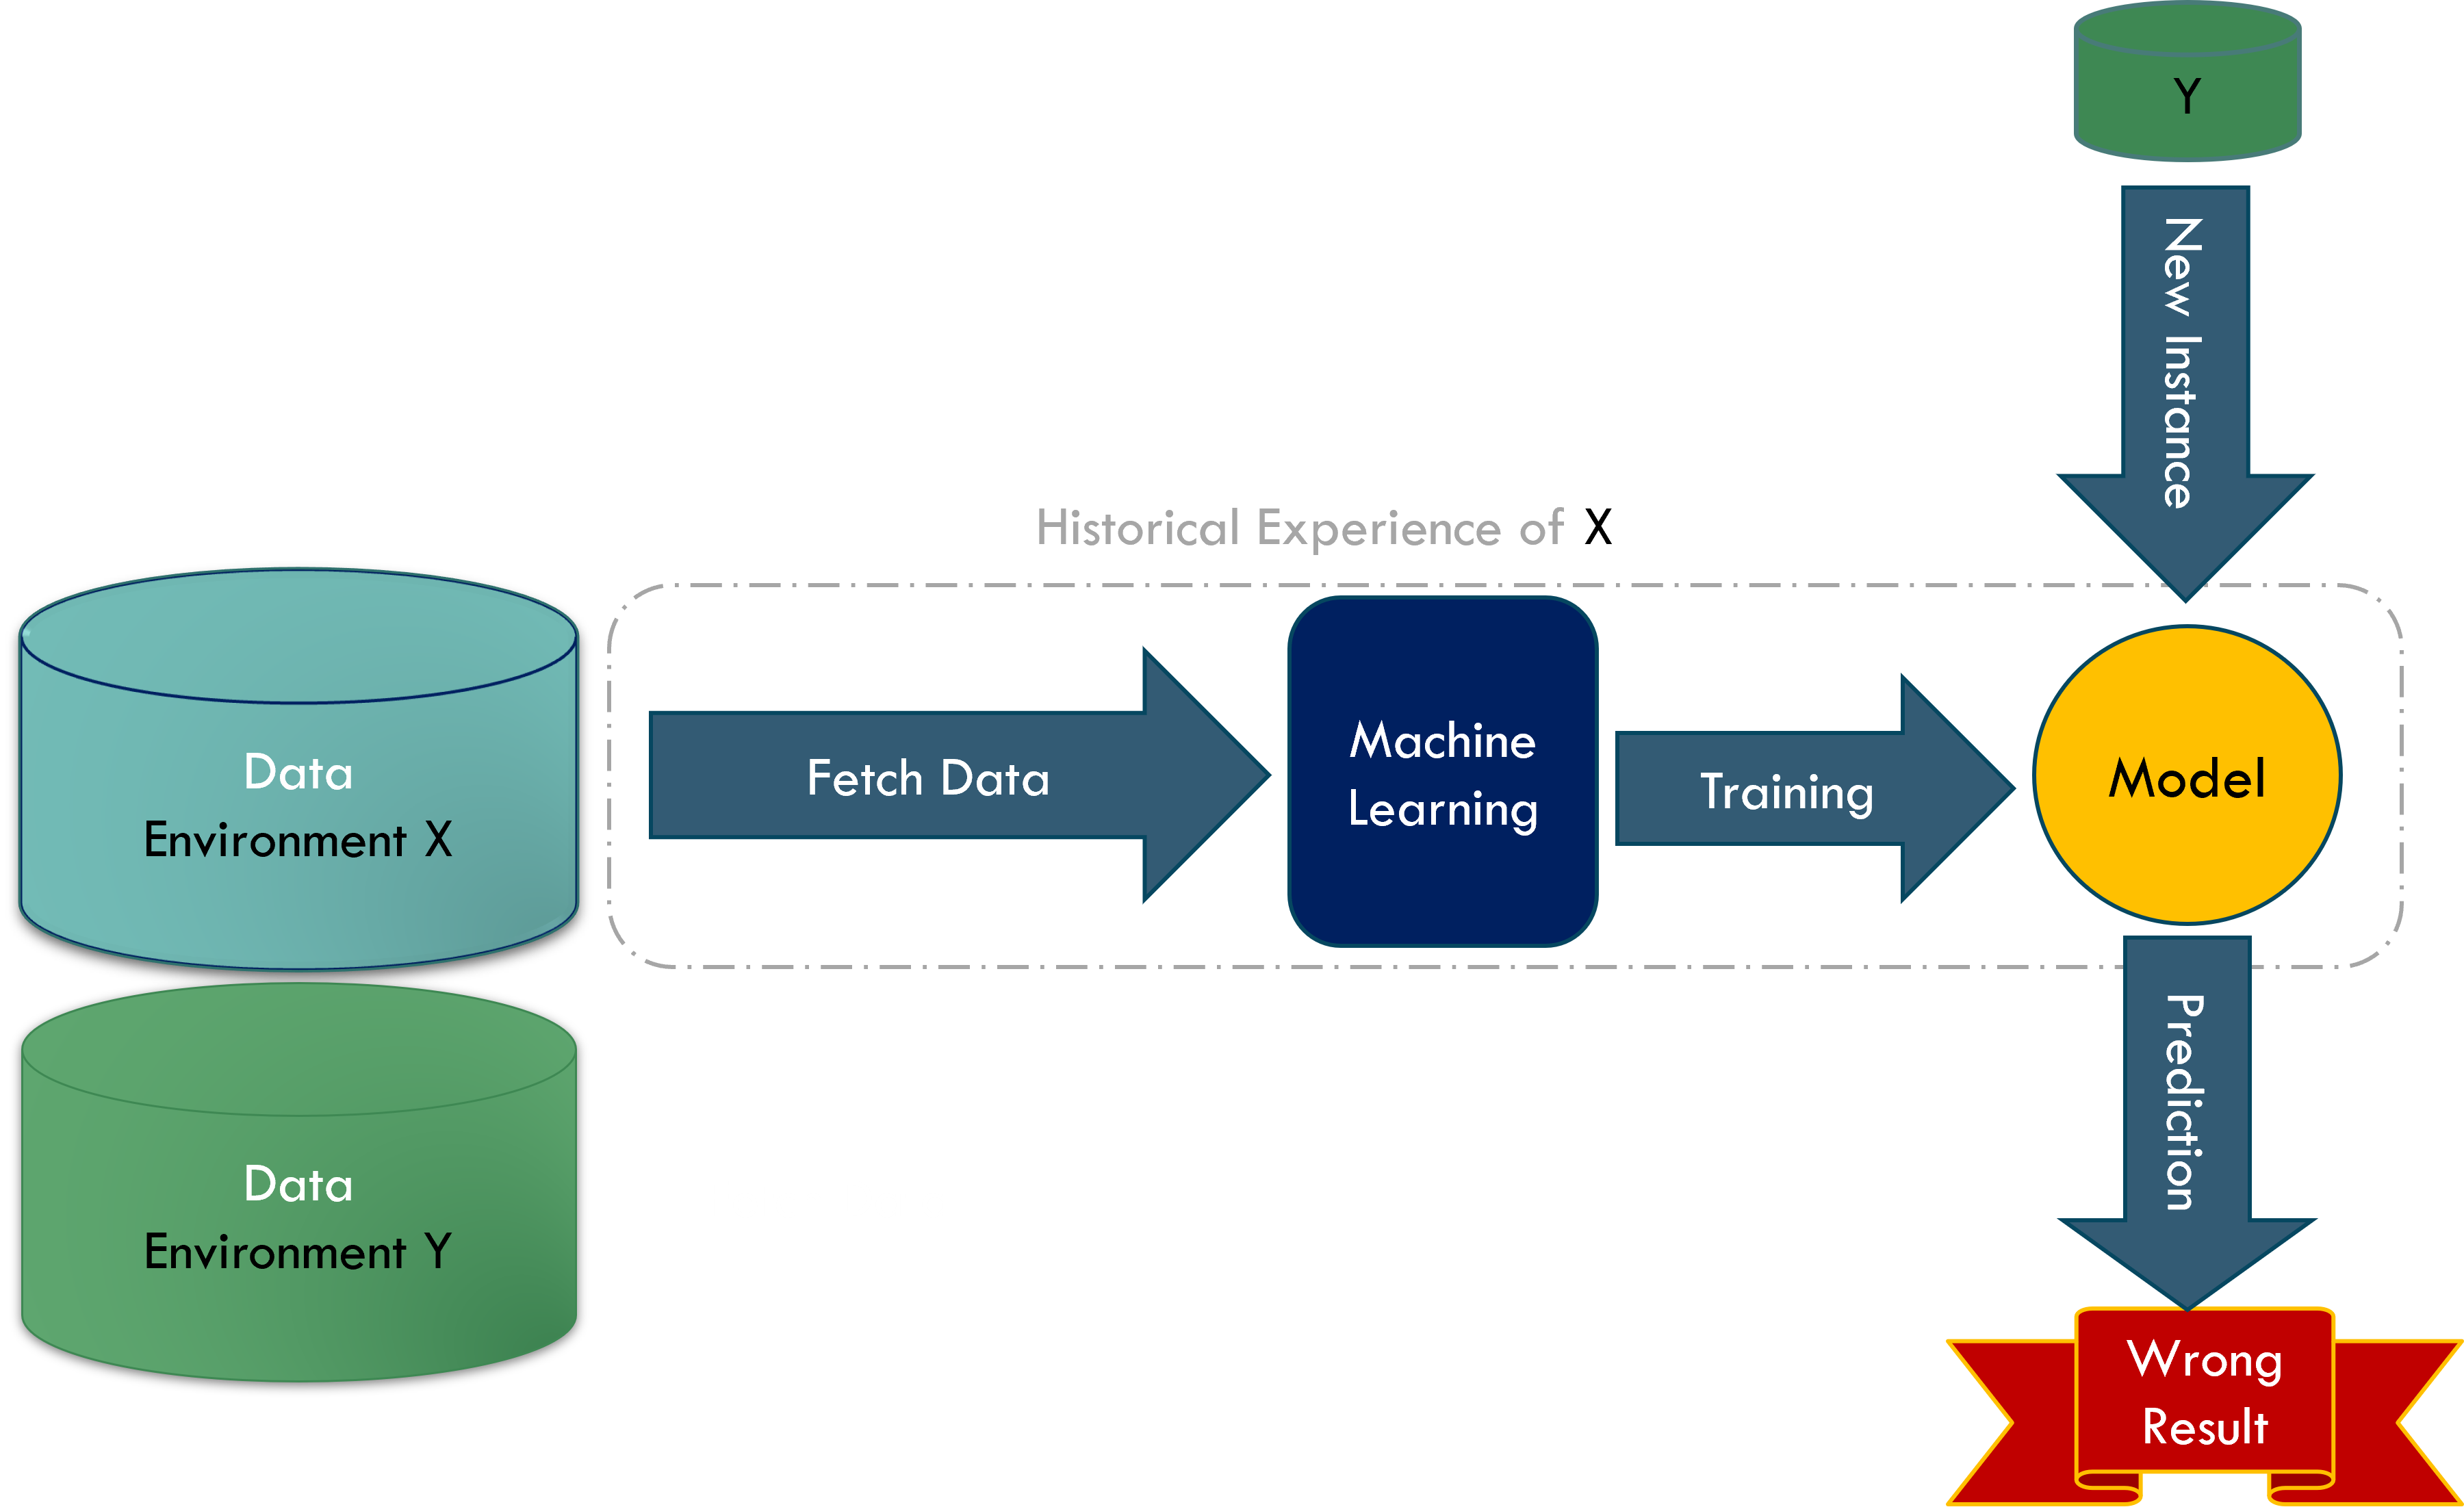
\includegraphics[width=.8\textwidth]{1_introduction/figures/PNG/wrong_machine_flow_1.png}\\
    (a) \\
    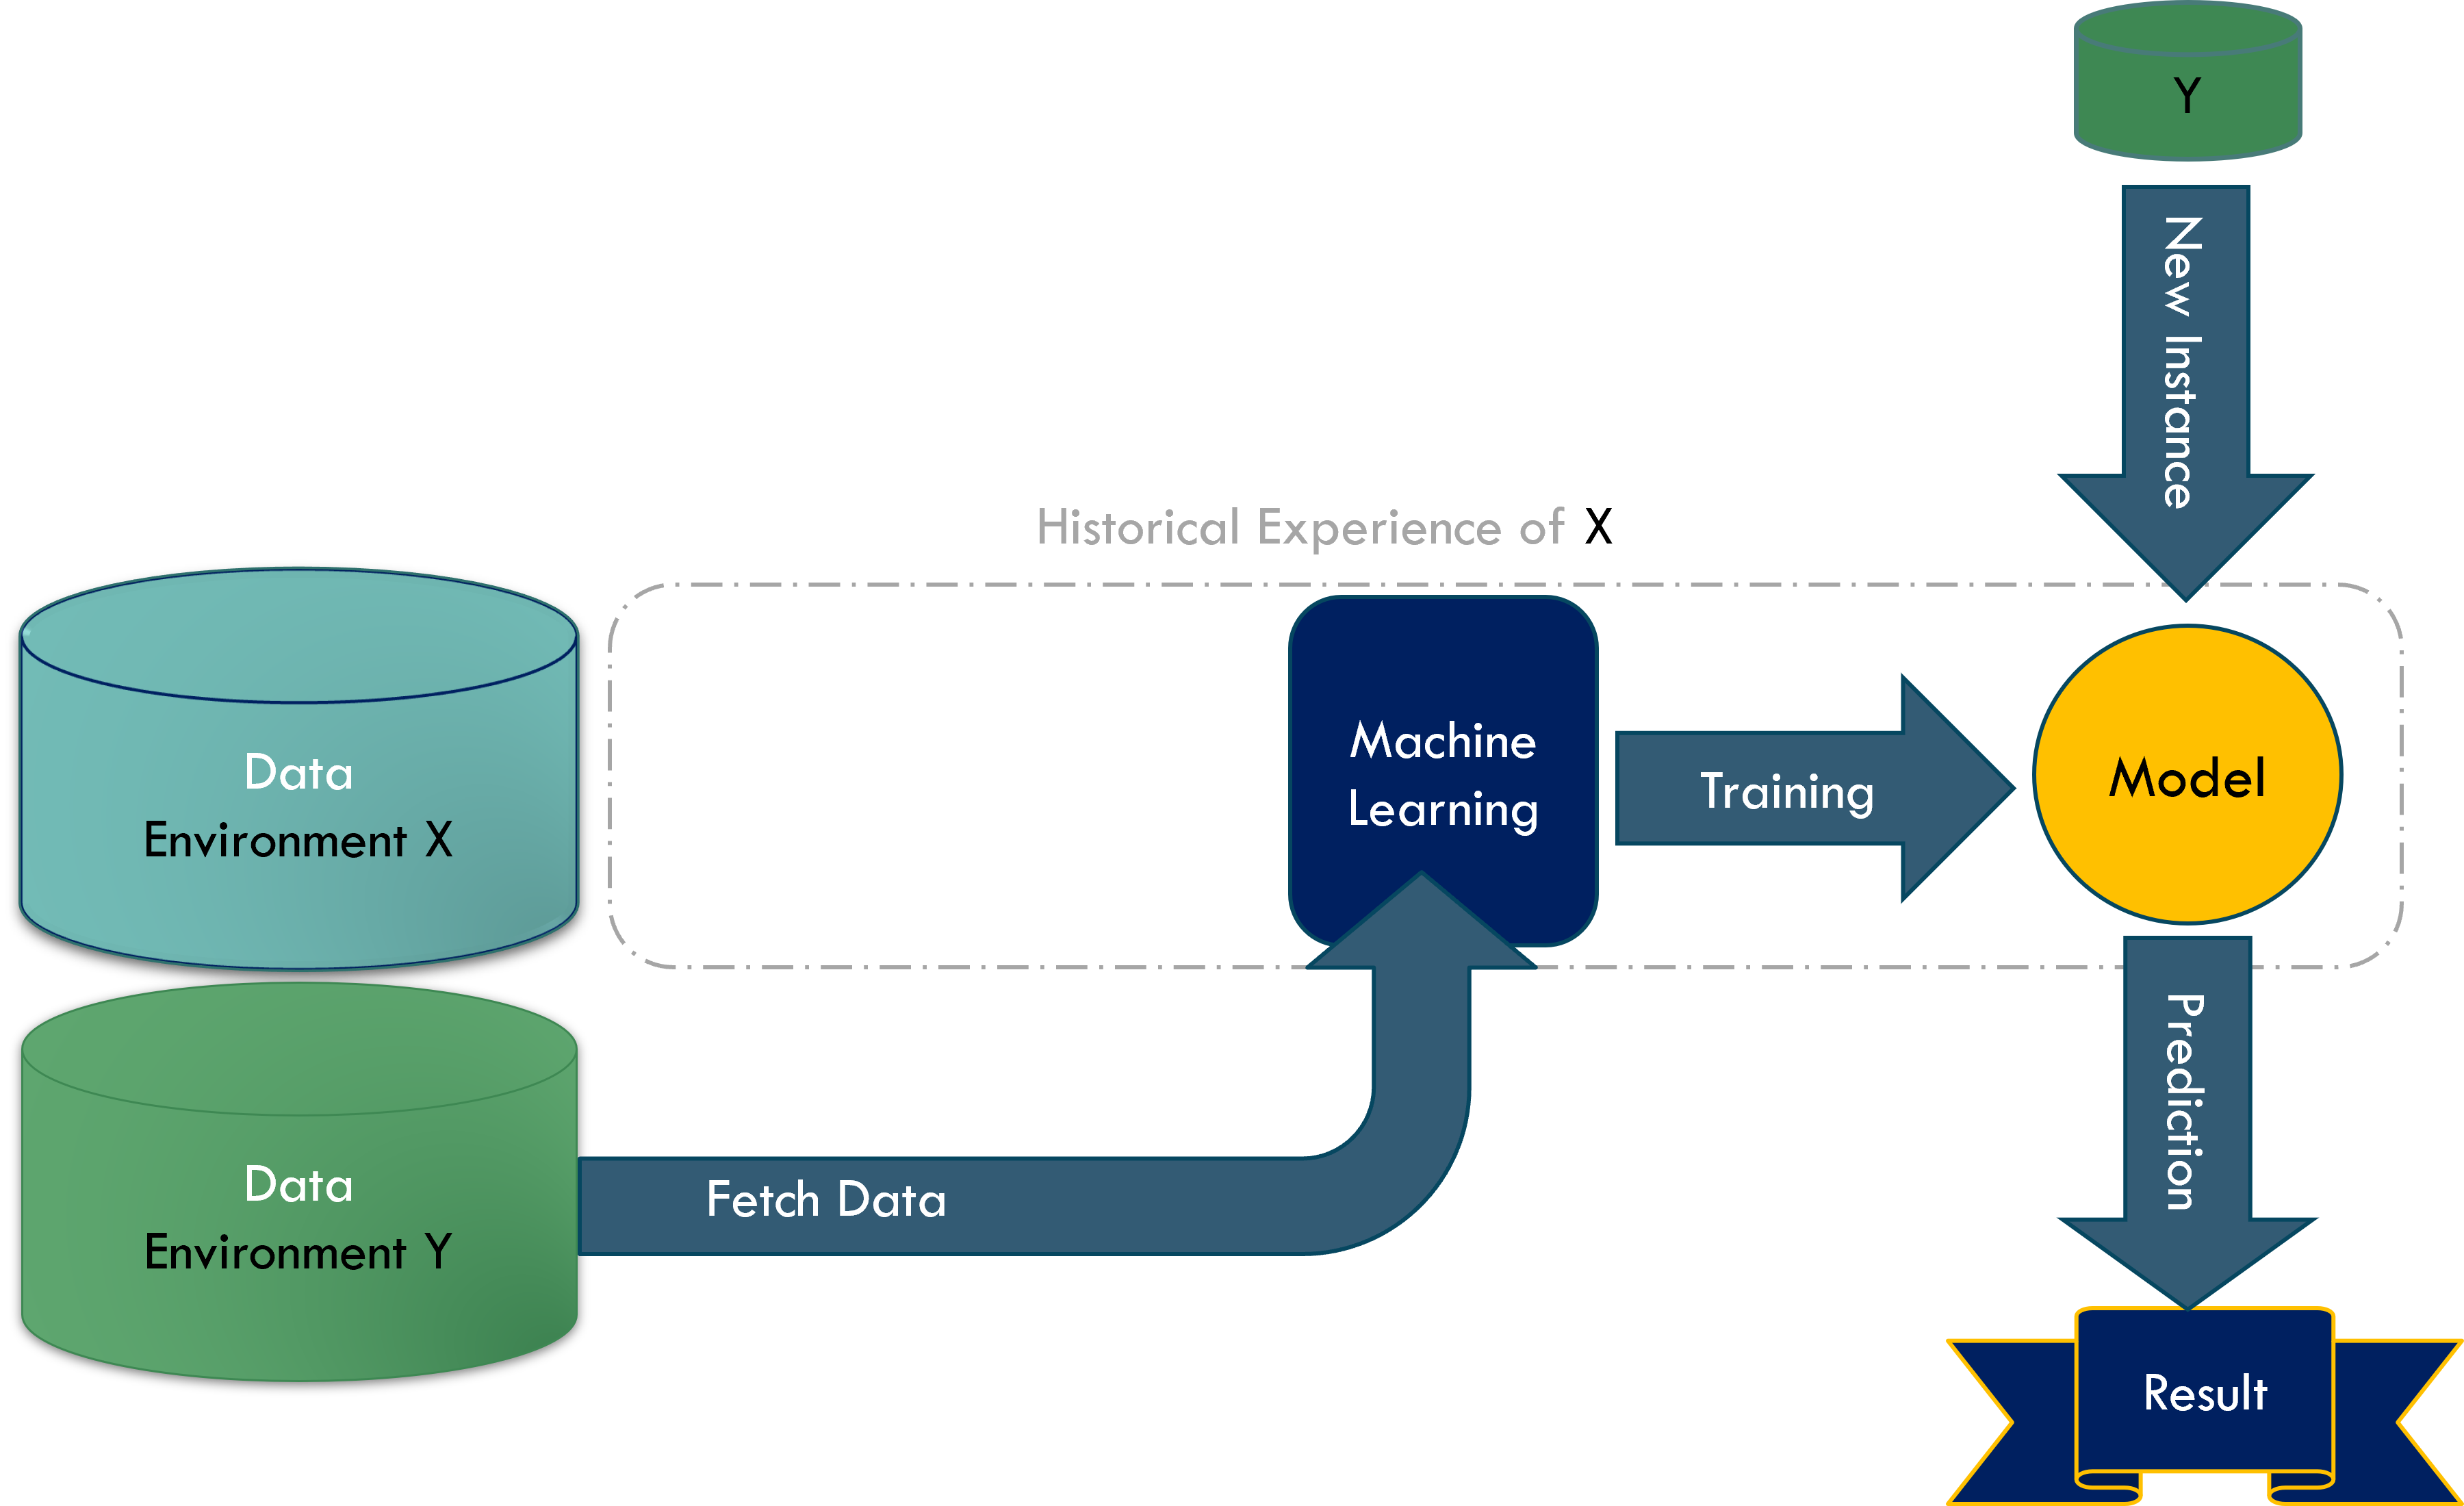
\includegraphics[width=.8\textwidth]{1_introduction/figures/PNG/wrong_machine_flow_2.png}\\
    (b)
    \caption{Machine Learning Workflow for Environment Y.}
    \label{fig:machine-new-senario}
\end{figure}



In recent years, high-speed data streams have presented significant challenges to machine learning models, particularly in streaming data analysis. These streams, characterized by continuous, dynamic, and high-volume data arrivals, demand adaptive learning algorithms to cope effectively with their evolving nature \cite{yang2021concept, dong2019multistream, shan2018online}. Among the critical challenges are concept drift, class imbalance, emerging new classes, and heterogeneous transfer learning.  

Concept drift refers to changes in the statistical properties of data over time \cite{pan2009survey, zhuang2020comprehensive}, which necessitates continuous adaptation of machine learning models. This phenomenon may manifest as shifts in underlying concepts, relationships between variables, or alterations in data distribution. Addressing concept drift involves employing detection mechanisms that monitor classifier performance or data distribution changes, triggering model updates, retraining, or replacement. These dynamic adjustments ensure model efficacy in the face of evolving data streams.  

Class imbalance and class overlap pose additional challenges, particularly in multi-class scenarios. Class imbalance, where data is unevenly distributed across classes \cite{wang2018systematic, sun2009classification}, often leads to misclassification of underrepresented classes. Techniques such as oversampling, undersampling, algorithm adaptation, and hybrid approaches have been employed to address these challenges \cite{charte2015addressing, charte2015mlsmote, daniels2017addressing, liu2018making}. Class overlap, where instances from different classes occupy the same data regions \cite{bhowan2012evolving, galar2011review}, complicates distinguishing between classes. Methods like class-overlap undersampling leverage local similarities to mitigate these issues.  

Dynamic classifier ensembles, particularly Dynamic Ensemble Selection (DES)  methods, offer solutions by adapting ensemble composition based on data characteristics \cite{cruz2018dynamic}. These methods optimize classifier subsets through criteria like diversity metrics and performance estimation, ensuring a balance between accuracy and computational efficiency \cite{kuncheva2000clustering}. DES approaches can dynamically select the most competent classifiers for each data instance \cite{woloszynski2011probabilistic, lysiak2014optimal, cruz2017meta}, enhancing classification in non-stationary streams.  

 Transfer learning  plays a pivotal role in addressing dynamic data streams and concept drift, focusing on leveraging knowledge from source domains to improve target domain learning \cite{pan2009survey, wang2018systematic}. Strategies include instance re-weighting, feature matching, and mitigating negative transfer effects to bridge domain gaps and improve adaptability.  

Finally, the challenge of  Streams with Emerging New Classes (SENC) involves scenarios where new classes, absent during initial training, emerge in data streams. Traditional models struggle to recognize and integrate these novel classes in real-time, necessitating adaptive learning mechanisms. This underscores the complexity of real-world data streams and highlights the importance of robust frameworks to manage such dynamics.  

Overall, addressing these challenges requires integrating dynamic ensembles, adaptive sampling techniques, and transfer learning to ensure accuracy and scalability in non-stationary data environments. Figures and citations support these discussions, emphasizing the critical need for adaptive solutions \cite{chawla2003smoteboost, wang2010negative}.
     
In this chapter, the problem definition for this research 
that naturally arise is discussed in  Section \ref{sec:1_introduction_problem}. After this, the the motivation is presented in Section \ref{sec:1_introduction_motivation} . After this, the objectives and
research contribution are presented in Sections \ref{sec:1_introduction_objectives} and \ref{sec:1_introduction_contribution}. Next, the research plan is summarised in Section \ref{sec:1_introduction_methodology}.  Finally, the outline of this thesis is presented in
\ref{sec:1_introduction_organizations}.